\section{Aggregated Subsector Dependency Network}
\label{sec:subsector_network}

This final structural summary translates retained ticker-level edges into a subsector-level map: nodes are subsectors and an edge is the average retained dependency between their constituent tickers. It is a descriptive aid for identifying concentrated or bridge-like connections, not a causal map or a new aggregation estimator. Figure~\ref{fig:subsector_network} and Table~\ref{tab:subsector_summary} report the resulting network. It contains 22 subsectors and 66 edges, with density 0.2857. The mean edge dependency is 0.0566 and the median edge dependency is 0.0561. These values are lower than typical raw asset-level correlations because the network summarizes filtered and aggregated dependencies rather than direct pairwise asset correlations.

The top-degree subsector is Retail, indicating broad direct connectivity in the aggregated dependency map. Electric Utility has the highest betweenness, suggesting that it occupies a bridge-like position in the subsector-level network. Apparel and Footwear has the highest weighted degree, reflecting stronger dependency intensity across its retained connections. These summaries help translate the ticker-level PMFG structure into economic language.

Table~\ref{tab:subsector_summary} gives the node-level details behind this interpretation. Degree measures how many of the 66 retained subsector links touch a given node, whereas weighted degree also accounts for the strength of those links. The two measures therefore need not identify the same subsector: a node may have many relatively weak connections or fewer but stronger ones. Betweenness identifies nodes that connect otherwise less-related parts of the graph, while internal mean dependency summarizes the average filtered dependency among assets belonging to the same subsector. For subsectors represented by a single asset, this within-subsector quantity is reported as zero because no within-subsector pair exists.

Figure~\ref{fig:subsector_network} provides the complementary structural view. Each node represents a subsector, its colour indicates the macro-sector, and its size is proportional to the number of assets in that subsector. The spatial layout is only a visualization of graph connectivity; distances between plotted nodes should not be interpreted as additional economic distances. Thick edges indicate larger average retained dependencies and make concentrated cross-subsector relationships visible, while bridge-like positions and peripheral nodes can be compared with the betweenness and degree values in Table~\ref{tab:subsector_summary}. Because the graph is built after ticker-level filtering and subsector aggregation, it should be read as a compact descriptive summary of the retained dependency structure, not as a causal or point-in-time network.

The subsector network motivates the exploratory retrospective model assessment that follows. It does not establish that centrality predicts future volatility: a real-time test would require the network to be reconstructed at each forecast origin.


\begin{center}
\captionof{table}{Subsector-level summary of the aggregated dependency network.}
\label{tab:subsector_summary}
\scriptsize
\resizebox{\linewidth}{!}{%
\begin{tabular}{llrrrrr}
\toprule
Subsector & Macro-sector & Assets & Degree & Weighted degree & Betweenness & Internal mean dep. \\
\midrule
Aerospace and Defense & Industrials & 1 & 4 & 0.1355 & 0.0381 & 0.0000 \\
Apparel and Footwear & Consumer Cyclical & 2 & 12 & 0.9412 & 0.0190 & 0.1676 \\
Banks & Financials & 5 & 5 & 0.2540 & 0.0786 & 0.0841 \\
Chemicals & Basic Materials & 3 & 6 & 0.2134 & 0.2833 & 0.0497 \\
Construction Materials & Industrials & 1 & 9 & 0.6055 & 0.0095 & 0.0000 \\
Electric Utility & Utilities & 10 & 4 & 0.1080 & 0.3310 & 0.1033 \\
Financial Services & Financials & 2 & 4 & 0.2911 & 0.0000 & 0.1096 \\
Gas Utility & Utilities & 1 & 5 & 0.2563 & 0.0190 & 0.0000 \\
Insurance & Financials & 1 & 7 & 0.3801 & 0.0190 & 0.0000 \\
Machinery and Equipment & Industrials & 3 & 8 & 0.4972 & 0.0571 & 0.0853 \\
Mining & Basic Materials & 3 & 4 & 0.3005 & 0.0190 & 0.2330 \\
Oil Gas and Biofuels & Oil Gas and Biofuels & 2 & 6 & 0.2602 & 0.1214 & 0.0714 \\
Paper and Cellulose & Basic Materials & 1 & 4 & 0.2082 & 0.0571 & 0.0000 \\
Personal and Home Care & Consumer Non-Cyclical & 1 & 5 & 0.2640 & 0.0048 & 0.0000 \\
Real Estate & Real Estate & 2 & 4 & 0.1561 & 0.0476 & 0.0093 \\
Retail & Consumer Cyclical & 2 & 13 & 0.8550 & 0.0667 & 0.1202 \\
Steel and Metallurgy & Basic Materials & 9 & 4 & 0.2513 & 0.0857 & 0.1161 \\
Telecommunications & Telecommunications & 2 & 4 & 0.1204 & 0.0714 & 0.7955 \\
Textiles & Consumer Cyclical & 1 & 7 & 0.4747 & 0.0476 & 0.0000 \\
Transportation & Industrials & 2 & 8 & 0.3689 & 0.3214 & 0.0428 \\
Transportation Equipment & Industrials & 2 & 5 & 0.3595 & 0.0000 & 0.0584 \\
Water and Sanitation & Utilities & 2 & 4 & 0.1738 & 0.0143 & 0.0691 \\
\bottomrule
\end{tabular}}
\end{center}
\noindent\footnotesize\emph{Notes:} The network contains 22 subsectors and 66 retained undirected links (density $0.2857$); its mean and median edge dependencies are $0.0566$ and $0.0561$. Degree counts retained subsector links, weighted degree sums their dependency weights, betweenness is the standard shortest-path measure on the aggregated graph, and internal mean dependency is calculated from asset pairs within each subsector. The edge weights $W_{ab}$ are defined in Section~\ref{subsec:subsector_network_method}.
\GlobalPrecisionNote

\normalsize

\begin{center}
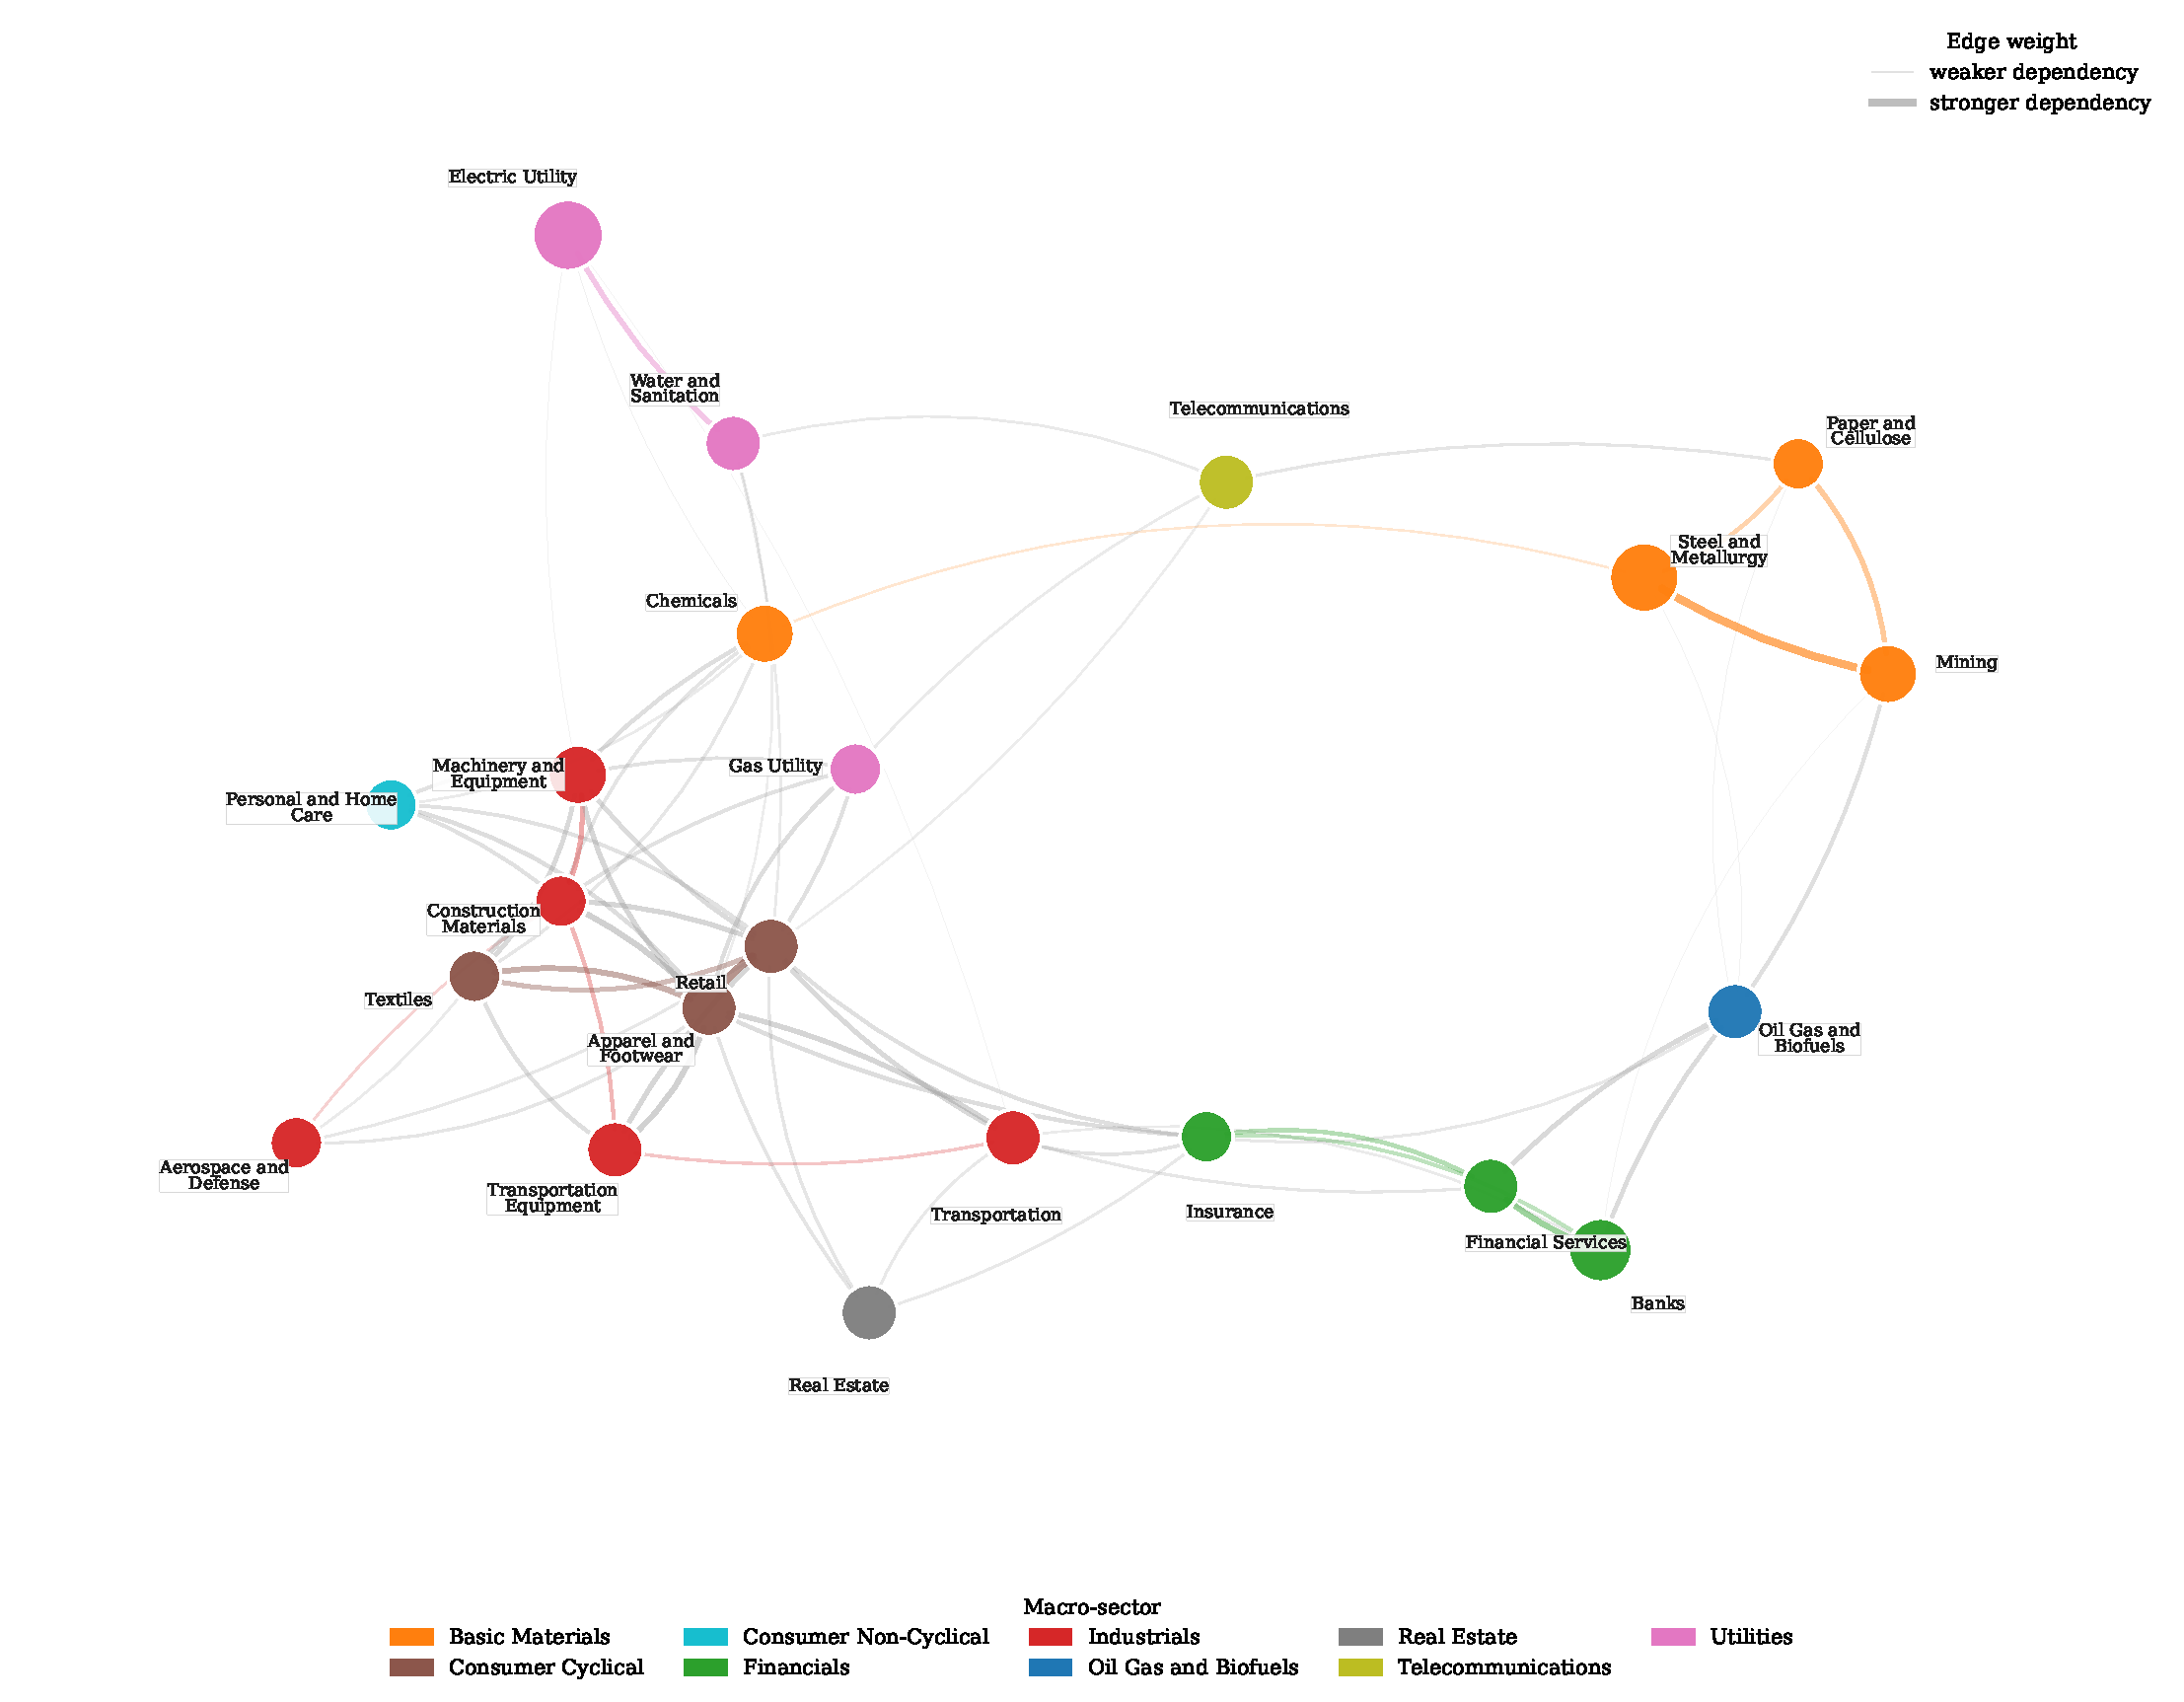
\includegraphics[
  width=0.92\linewidth,
  height=0.58\textheight,
  keepaspectratio
]{images/figure_15_subsector_dependency_network.pdf}
\captionof{figure}{Aggregated subsector dependency network. Nodes represent subsectors, node colour identifies the macro-sector and node size is proportional to the number of assets in the subsector. Edges represent retained subsector-level dependency weights, with thicker edges indicating stronger average dependency.}
\label{fig:subsector_network}
\end{center}
